\documentclass[tikz]{standalone}
\usetikzlibrary{intersections}
\begin{document}
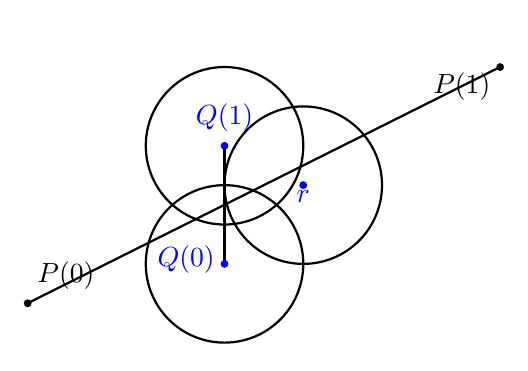
\begin{tikzpicture}
  \useasboundingbox (0,3.5) rectangle (6,-0.5);
  \coordinate (e1) at (0, 0);
  \coordinate (e2) at (6, 3);
  \coordinate (u)  at (2.5,  0.5);
  \coordinate (q1)  at (2.5,  2);
  \coordinate (v)  at (3.5, 1.5);

  \draw[thick] (e1) -- (e2);
  \draw[thick] (u) -- (q1);

  \draw[thick] (u) circle (1);
  \draw[thick] (q1) circle (1);
  \draw[thick] (v) circle (1);

  \path[name path=line] (e1) -- (e2);
  \path[name path=circleu] (u) circle (1);
  \path[name path=circleu] (q1) circle (1);
  \path[name path=circlev] (v) circle (1);
  \path[name intersections={of=line and circleu, by={tu1,tu0}}];
  \path[name intersections={of=line and circlev, by={tv1,tv0}}];

  \node[circle,fill,color=black,inner sep=1pt,label={[text=black, above right]:\(P(0)\)}] at (e1) [] {}; 
  \node[circle,fill,color=black,inner sep=1pt,label={[text=black, below left]:\(P(1)\)}] at (e2) [] {}; 

  \node[circle,fill,color=blue,inner sep=1pt,label={[text=blue, left]:\(Q(0)\)}] at (u) [] {}; 
  \node[circle,fill,color=blue,inner sep=1pt,label={[text=blue, above]:\(Q(1)\)}] at (q1) [] {}; 
  \node[circle,fill,color=blue,inner sep=1pt,label={[text=blue, below]:\(r\)}] at (v) [] {}; 
\end{tikzpicture}
\end{document}
